% Capítulo 6
\chapter{Estudo Experimental Preliminar}
\label{cap:cap6}

Este capítulo consiste em apresentar o estudo experimental realizado, refere-se ao processo de validação preliminarmente da taxonomia proposta e envolve a concepção do contexto de experimentação, das configurações e características dos elementos envolvidos, a seleção das variáveis influenciadoras, o controle e instrumentalização do experimento, sua execução e captura de dados durante experimentação, e por fim, a análise e indícios encontrados obtidos a partir desses resultados. 

O objetivo do experimento é analisar por meio de demonstração da taxonomia proposta, a atuação de mecanismos \textit{throttling}, como candidato atuante no incremento da disponibilidade dos elementos presentes em \textit{IoT} através da adaptação de comportamento por ação de limiares que considerem seus aspectos energéticos para assim,  prolongar a autonomia energética dos dispositivos. A abordagem é aderente e cobre os elementos presentes na taxonomia definida no Capítulo \ref{cap:cap4}, permitindo comparação e análise entre dispositivos que diferem sobre o fato de terem sua operação ajustada mediante \textit{throttling} ou não. 

\section{Metodologia}

O experimento compara os efeitos do mecanismo de \textit{throttling} em dispositivos com capacidade de coleta de energia, com foco em examinar os indícios de incremento na disponibilidade de cada um voltado aos aspectos energéticos em condições de atuação semelhante.

\begin{figure}[H]
	\centering
	\caption{Processo de Estudo Experimental.}
	\label{fig:cap6metodologia}
	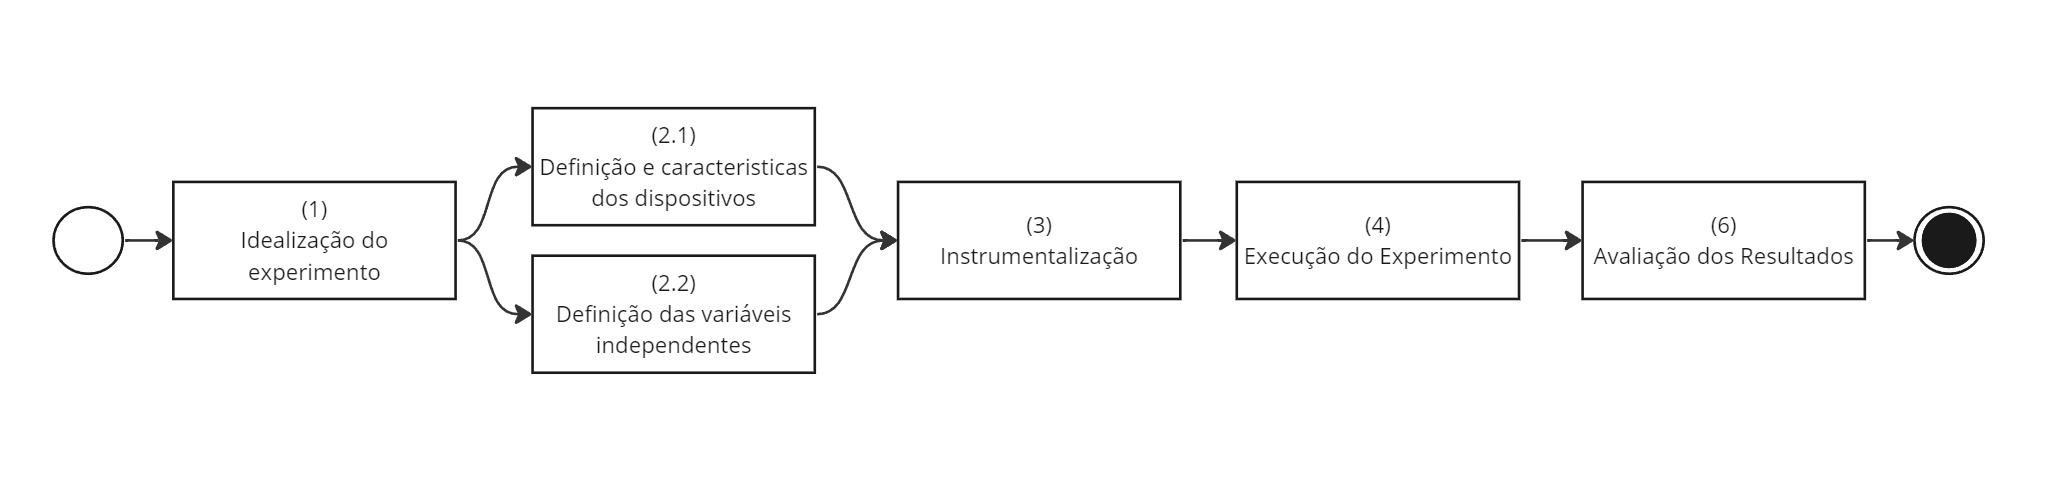
\includegraphics[width=1\linewidth]{Imagens/cap6/cap6metodologia.jpg}
	
	Fonte: elaborado pelo autor.
\end{figure} 

Para tal, buscou-se observar a influência do fator limitante na alteração do comportamento dos dispositivos participantes em resposta aos valores referentes à energia coletada e, consequentemente, à sua reserva energética. Além disso, pretende-se compreender o processo realizado para tomada de decisão sobre atender ou não às solicitações, baseando-se na análise das capacidades do dispositivo à medida que varia a oferta energética disponível. Este estudo visa categorizar os agentes envolvidos no processo de implementação do \textit{throttling} como solução para estender a disponibilidade dos dispositivos em relação aos fatores energéticos, focando na capacidade de coleta energética.

A Figura \ref{fig:cap6metodologia} apresenta os processos executados e sua ordem exprime a precedência para realização das etapas adjacentes. Na Seção \ref{cap6:idealizacao}, foi concebido a idealização do experimento (Etapa 1), quais os requisitos do estudo para viabilizar a análise e comparação de dispositivos com diferentes instanciações do \textit{throttling} buscando à cobertura das categorias taxonômicas definidoras. Partindo daí, foi projetado um ambiente para abstrair os elementos envolvidos, buscando garantir o controle na equidade de condições para os dispositivos observados. Todo o processo foi concebido e viabilizado pelo uso da plataforma Docker\footnote{Disponível em \url{https://www.docker.com/}.}, uma plataforma de virtualização que atua sobre o desenvolvimento, envio e execução de aplicativos organizados na forma de contêineres e por esses fatores, atende às restrições necessárias de encapsulamento para cada aplicação e suas dependências auto contidas.  

A abordagem utilizando \textit{containers} permitiu que os dispositivos fossem estimulados simultaneamente, mantendo controle sobre seus recursos garantindo os termos da operação, garante equidade de condições semelhante à dispositivos \acs{IoT} encontrados em um ambiente. Sendo assim, a definição dos dispositivos e variáveis (Etapa 2) do experimento considera:  I - Os dispositivos foram instanciados apenas sob o ponto de vista das classes taxonomicas definidas; II - Dispositivos simulados com capacidade de coleta e armazenamento de energia estão inseridos em um dado ambiente similar ao uso real; III - Os dispositivos recebem, ao mesmo tempo, um valor como coleta de energia; IV - Os dispositivos participantes possuem a mesma capacidade para armazenar energia coletada em \textit{storage}; V - Os dispositivos são submetidos ao mesmo tipo de solicitações simultaneamente.

Na Instrumentalização (Etapa 3), capacita o experimento para coletar, apresentar e preservar os resultados aferidos de uma execução e posterior visualização dos dados obtidos, os detalhes estão descritos na Seção \ref{cap6:instrumentalizacao}. A Seção \ref{cap6:execucao} descreve apropriadamente os detalhes de execução (Etapa 4). Neste ponto, todas as etapas planejadas anteriormente no andamento do processo ja foram abordadas. Em decorrência disso, habilita-se o experimento para realizar múltiplas execuções conforme protocolo estabelecido, aplicando os estímulos observáveis, necessários em conformidade com a análise das soluções encontradas no porftólio para o estudo. Uma vez definidos, carga de solicitações em ciclos e disponibilização de recursos energéticos, coleta-se os resultados obtidos para análise.

Em seguida, a Seção \ref{cap6:avaliacao}, apresenta a avaliação dos resultados (Etapa 5), que consiste na descrição e análise dos dados obtidos durante a execução. Os dados analisados são compostos pelos valores inferidos ao grupo de variáveis independentes e os resultados obtidos no grupo de variáveis dependentes. Constituem as variáveis independentes: os valores energéticos disponibilizados; e da quantidade de solicitações realizadas. A análise é fundamentada em observar como o mecanismo \textit{throttling} implementado no dispositivo se colocará como agente atenuante do gasto energético utilizado a medida seus limiares de atuação são atingidos de acordo com o modo de operação previsto para determinados fatores observáveis presentes. 

Finalmente, esta avaliação pretende observar a completude da cobertura obtida pelas classes taxonômicas enquanto necessárias para caracterizar o uso do \textit{throttling} em dispositivos \acs{IoT} para computação dirigida à energia. Por isso, encerrando a execução do experimento, as variáveis dependentes resultantes são coletadas para avaliação e evidenciam: como o limitador impacta em performance na relação a quantidade total de solicitações atendidas em igualdade de ciclos entre diferentes dispositivos e das  condições de indisponibilidade para realizar operações mediante esgotamento dos recursos em \textit{storage}.  Ao aprofundar a análise, é preciso ainda, contrapor os dados temporais de oferta energética em relação a quantidade presente no dispositivo, observando indícios da atuação de limitadores e sua capacidade em manter um dispositivo operacional do ponto de vista energético.


\section{Idealização}
\label{cap6:idealizacao}
Uma vez definido os objetivos do experimento, a idealização é o ponto onde foi construído as bases de execução do estudo. Assim, foram concebidas a estruturação geral dos parâmetros, a  definição do cenário para realizar os testes, além da capacidade de coleta dos resultados e avaliação de conformidade com os termos presentes na taxonomia proposta.

O cenário foi idealizado para simular a atuação de dispositivos \acs{IoT} em computação dirigida à energia, presentes em dado ambiente, estes limitam-se as categorias da taxonomia definidas.  Aqui, fundamentalmente, as classes Agente, Operações e Recursos Energéticos estão em evidência. Os dispositivos enquanto agentes provedores devem atender as solicitações de operações à medida que são providos energeticamente por seu sistema de coleta (\textit{power supply}). Decorrente disso, cabe ao dispositivo, com base nas condições energéticas observado em seu armazenamento (\textit{storage}), decidir se é capaz ou não de realizar a operação solicitada. 

Para sua concepção é preciso definir temas travessais às categorias, se colocando termos auxiliares que colaboram para o processo experimental. Assim descreve-se \( C_a \) como o valor de consumo do dispositivo quando estado ativo, \( C_i \), o consumo enquanto estado inativo e \( C_h \) representa dispositivos sem capacidade energética, com seu valor é zero e configura um equipamento em estado hibernativo. 

Sobre o tempo a duração de um ciclo $T(c)$, os trabalhos abordados atribuem seu valor através da soma da duração do tempo dentro do ciclo onde o dispositivo esta ativo \( t_a \), permanece inativo \( t_i \) além do tempo que hiberna \( t_h \), é seguro expressar o tempo total do ciclo em razão dos constituintes na expressão $T(c_n) = $ \( t_a + t_i + t_h \). O consumo total $C_{total}$, durante um ciclo é obtido de maneira que:
\[C_{total} = C_a \cdot t_a + C_i \cdot t_i + C_h \cdot t_h \quad (\text{Sendo }C_h = 0)\]
\[C_{total} = C_a \cdot t_a + C_i \cdot t_i\]
Assim, considerando um dispositivo que permaneça ativo durante todo o ciclo \( t_a = T \), \( t_i = 0 \), \( t_h = 0 \):
\[ C_{total} = C_a \cdot T \]
De outra forma, caso permaneça hibernando durante todo o ciclo \( t_h = T \), teremos seu consumo total:
\[ C_{total} = C_h \cdot T = 0 \]

Portanto, um dispositivo com ação do mecanismo \textit{throttling} deverá ter seu comportamento adequado ao modo de atuação esperado, estimado em \acs{SLA}, através da recusa de solicitações durante os ciclos, proporcionando a variação entre $ t_a, t_i \ e\ t_h$ buscando cooperar com o motivo de atuação ou seja, para consumir seus recursos eficientemente, assim conduz o dispositivo ao cenário onde o tempo de atividade é cada vez menor ao tempo total do ciclo \( t_a < T \) enquanto, se necessário, manter $t_h \approx 0$.

Ainda nesta etapa, foi necessário conceber uma configuração de componentes adequadas que pudessem representar um dispositivo com capacidade de coleta energética. Com base na taxonomia proposta no Capítulo \ref{cap:cap4}, reduziu-se o dispositivo aos aspectos de armazenamento (\textit{storage}), sua entrada energética simulando um valor coletado através de um \textit{power supply}, sendo os demais componentes travessais para uma operação. Assim, a dinâmica energética segue-se ao passo que um valor energético é apresentado em ciclos ao \textit{storage}, que armazena e fornece os valores para uso dos demais componentes presentes. A Figura \ref{fig:cap6dinamica} ilustra dinâmica energética de funcionamento do dispositivo.

\begin{figure}[H]
	\centering
	
	\caption{Dinâmica do fornecimento energético Dispositivo Provedor.}
	\label{fig:cap6dinamica}
	\noindent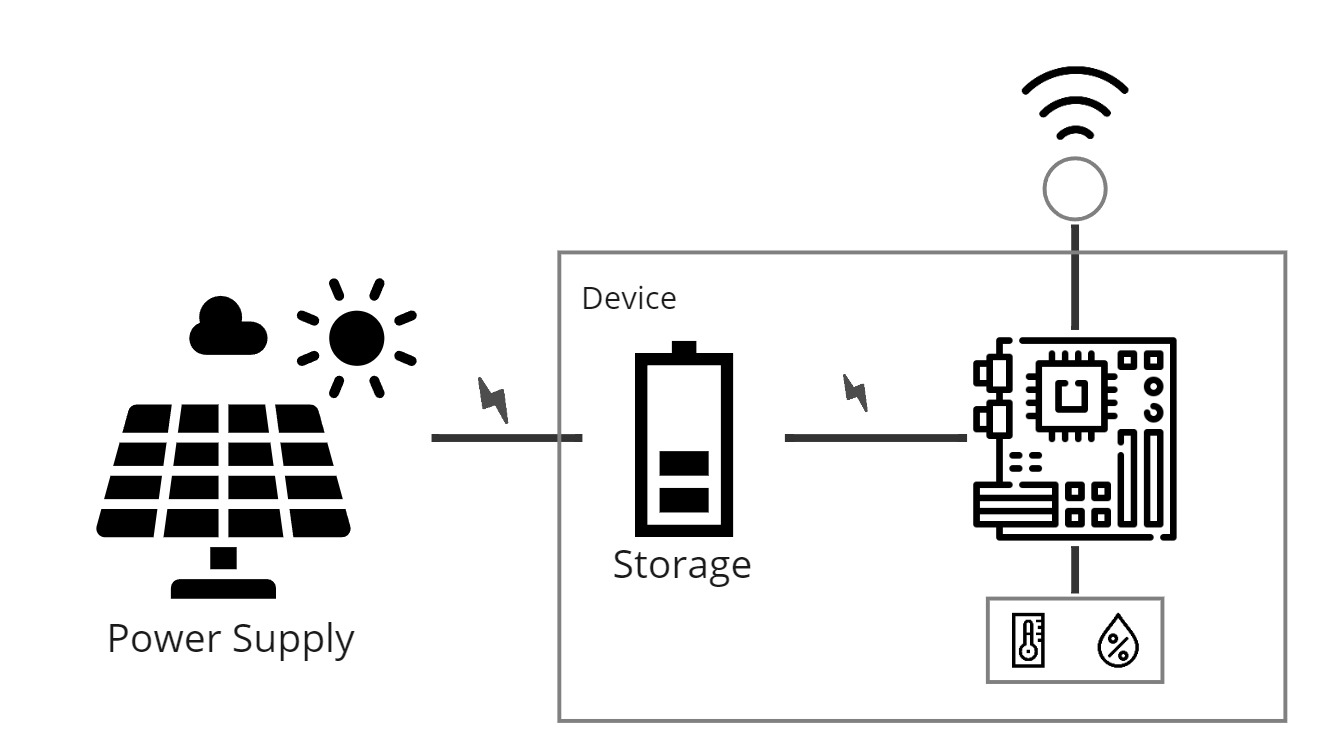
\includegraphics[width=0.75\linewidth]{Imagens/cap6/cap6dinamica.jpg} 
		
	Fonte: elaborado pelo autor.
\end{figure}


Em consequência, acontecendo disponibilidade energética, cabe ao dispositivo armazena-la na medida que os valores vão sendo apresentados, respeitando sua capacidade de armazenamento. Ao passo que paralelamente, os valores energéticos estão disponibilizados na forma de recurso ofertado e utilizado na medida que realiza suas operações.

Finalmente, o dispositivo deverá em todo seu funcionamento atuar dinamicamente em conformidade com os modo de operação projetados de acordo com um \acs{QoS} presente em seu acordo de nível de serviço, o qual faz referencia aos valores de recursos energéticos que possui. No experimento estão cobertos quatro modos de atuação a depender das capacidades energéticas:

\begin{enumerate}	
\item Modo Abundante:  representa o dispositivo que possui recursos energéticos amplamente disponíveis, permitindo o funcionamento completo e otimizado de todas as suas funcionalidades. Aqui, atenderá quaisquer solicitação enviada, sem atuação do mecanismo limitante, aproveitando ao máximo a disponibilidade de energia;
\item Modo Atenção: Uma vez atingido este patamar, o dispositivo ainda apresenta condição energética razoável, porém moderadamente restringirá algumas operações atendidas com a motivação de preservar parte dos recursos até que um novo cenário energético seja apresentado;
\item Modo Alerta: alcançado quando o dispositivo está operando com recursos energéticos extremamente limitados. Algumas operações ainda podem ser realizadas (conforme privilégios das operações ou solicitantes). Este modo motiva-se na intenção de prolongar a funcionalidade básica do dispositivo a todo custo enquanto tenta evitar a entrada no Modo Hibernação. 
\item Modo Hibernação: este modo é ativado quando não possui mais recursos energéticos disponíveis para realizar solicitações. O dispositivo entrará em um estado de hibernação ou equivalente até que recursos energéticos sejam recuperados. As ações que ocorrem nesse modo, são consideradas criticas para manutenção do estado do dispositivo, caso hiberne. Além disso, pode representar um dispositivo esgotado energeticamente, nesse caso, o dispositivo não realizará nenhuma operação.
\end{enumerate}

Um modo de operação guiará como o mecanismo de \textit{throttling} interpreta os observáveis, no experimento, tem atenção sobre o valor disposto em sua reserva energética, assim poderá contribuir reduzindo a utilização dos recursos, amortizando ou interrompendo o uso energético nos serviços ofertados no dispositivo a medida que limita à capacidade de atendimento as solicitações. 

Naturalmente, uma definição sobre os modos de operação deve sofrer variação, cabe a análise das especificidades e natureza que se destina cada implementação, para assim, dado o exame desses fatores, definir apropriadamente quais modos serão necessários para o dispositivo almejado. Estes modos guiam a capacidade de mudança dos estados do dispositivo. Uma vez que, são justificados por tal modo reduzindo as capacidades do dispositivo sobre quantidade de solicitações atendidas nos ciclos, proporcionando momento em estado de inatividade forçada contribuindo para restabelecimento ou conservação dos recursos. De maneira geral, a dinâmica dos estados do dispositivo pode ser visualizada na Figura \ref{fig:cap6maquinaestados}. 

\begin{figure}[H]
	\centering
	
	\caption{Máquina de estados do Dispositivo.}
	\label{fig:cap6maquinaestados}
	\noindent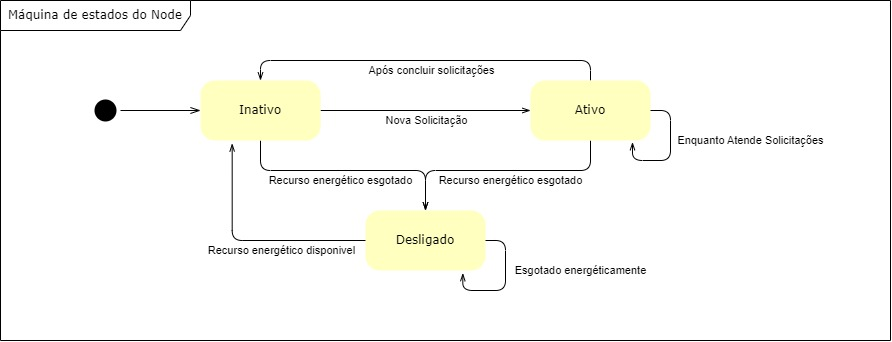
\includegraphics[width=0.75\linewidth]{Imagens/cap6/cap6maquinaestados.jpg} 
	
	Fonte: elaborado pelo autor.
\end{figure}

A relação entre modos de operação e estados também deixa explicita presença de mecanismo limitante mediante limiares definidos em cada modo, contribuindo para que o dispositivo permaneça em um estado de inatividade à depender das condições observadas com a motivação de preservar ou restabelecer sua condição. Sendo assim, uma vez identificado em um modo de operação, o dispositivo terá uma quantidade potencial para atendimento das operações durante os ciclos e estas, colocam o dispositivo em um estado ativo. Caso atinja valor limitador de acordo com o modo, novas operações passam a ser negadas e por sua vez, colocará dispositivo em inatividade, reduzindo assim seu gasto energético.

Para fins da experimentação, os estados possíveis para o dispositivo foram descritos como:
\begin{itemize}

	\item Estado Ativo: Um dispositivo é considerado ativo enquanto atende solicitações. Nesse estado o dispositivo utilizará os recursos energéticos necessários para realização das atividades mediante o consumo desses recursos. 
	
		\item Estado Hibernando: No experimento, o estado hibernando é a indicação que o dispositivo não tem mais capacidade de assumir qualquer outro estado enquanto não receber recursos energéticos, seja por modo contundente de preservação ou em decorrência do esgotamento de suas reservas. Portanto, neste estado, um dispositivo não realizará qualquer atividade.

	\item Estado Inativo: Aqui o dispositivo estará consumindo a menor quantidade de recurso energético possível. Enquanto inativo, encontra-se ocioso sem realizar nenhuma tarefa à medida que aguarda novas solicitações ou seja o caso necessário, aguarde nova entrada energética disponível, para atender solicitações anteriormente recusadas. Alguns estudos apontam que o estado inativo pode ser suprimido, restando apenas os estados Ativos e Hibernando (\textit{Sleep, Wake}) como os utilizados em (\citeonline{gong_sleep_2022}; \citeonline{luo_optimal_2017}), em todo caso o estado inativo pode ser contemplado a depender da aplicação e necessidades apresentadas aos dispositivos \acs{IoT}.
	
	
	
	
\end{itemize}




\section{Definição das Variáveis Independentes}
\label{cap6:variaveisdispositivos}
Dispositivos com a capacidade de coleta de energia (\acl{EHS}) se baseiam na utilização de fontes energéticas disponíveis no ambiente para suprir, parcial ou totalmente, a demanda de um dispositivo. Esta caracteristica é fundamental para os dispositivos em computação dirigida à energia. Em todo caso, para o experimento, não há, a princípio, a intenção de analisar as particularidades do processo de obtenção de recursos de alguma fonte energética, sua natureza e características de uso ou eficiência. 

Todavia, na execução do experimento é necessário a compreensão sobre à disponibilidade da oferta energética em termos quantitativos de uma fonte qualquer, Pois com isso, busca-se conduzir o experimento aos critérios utilizados nas abordagens estudadas e por sua vez, categorizados taxonomicamente em respeito à capacidade de coleta do dispositivo, assim os dados utilizados se assemelham ao comportamento observado por um fonte de energia solar e foram concebidos à partir de adaptação dos dados reais disponibilizados no Atlas Brasileiro de Energia Solar \cite{martins2017atlas}. Em destaque, a definição dos valores foi orientada pela referencia para cidade de Natal/RN como média diária de irradiação solar no decorrer dos meses. Adaptado ao experimento, cada valor apresentado compreenderá à uma jornada $J_i$ (para $i = 1,2,...,12$), uma execução realizada integralmente durará 12 jornadas. Para viabilizar o experimento, os valores originários foram tratados como parâmetro de quantidade apenas, desprezando sua grandeza. Assim,  Conforme Tabela \ref{table:cap6distribuicaonatal}, cada valor representa o montante energético disponibilizado em uma respectiva jornada distribuídos em ciclos.

\begingroup

\setlength{\tabcolsep}{10pt} % Default value: 6pt
\renewcommand{\arraystretch}{1.5} % Default value: 1

\begin{table}[h]
	
	\centering
	\caption{Valores ofertados por ciclo}
	\smaller[8]
	\tabcolsep=0.1cm
\begin{tabular}{ r | *{13}{c} }
	\toprule
        &  \multicolumn{13}{c}{Disponibilizado no Ciclo (c)}\\\cline{2-14}
	Jornada (J) & \begin{tabular}{@{}c@{}} c05 \\(0.007)\end{tabular} &
	\begin{tabular}{@{}c@{}} c06 \\(0.02) \end{tabular}	& 
	\begin{tabular}{@{}c@{}} c07 \\(0.053)\end{tabular} &
	\begin{tabular}{@{}c@{}} c08 \\(0.087) \end{tabular}&
	\begin{tabular}{@{}c@{}} c09 \\(0.105) \end{tabular}&
	\begin{tabular}{@{}c@{}} c10 \\(0.127) \end{tabular}& 
	\begin{tabular}{@{}c@{}} c11 \\(0.136) \end{tabular}& 
	\begin{tabular}{@{}c@{}} c12 \\(0.125) \end{tabular}& 
	\begin{tabular}{@{}c@{}} c13 \\(0.12) \end{tabular}& 
	\begin{tabular}{@{}c@{}} c14 \\(0.101) \end{tabular}& 
	\begin{tabular}{@{}c@{}} c15 \\(0.074)\end{tabular}& 
	\begin{tabular}{@{}c@{}} c16 \\(0.04)\end{tabular}&
	\begin{tabular}{@{}c@{}} c17 \\(0.005)\end{tabular}\\
	
	\hline
	J01 5674 & 39.72 & 113.48 & 300.72 & 493.64 & 595.77 & 720.6 & 771.66 & 709.25 & 680.88 & 573.07 & 419.88 & 226.96 & 28.37\\
	\hline
	J02 6017 & 42.12 & 120.34 & 318.9 & 523.48 & 631.78 & 764.16 & 818.31 & 752.12 & 722.04 & 607.72 & 445.26 & 240.68 & 30.09 \\
	\hline
	J03 6032 &  42.22 & 120.64 & 319.7 & 524.78 & 633.36 & 766.06 & 820.35 & 754.0 & 723.84 & 609.23 & 446.37 & 241.28 & 30.16 \\
	\hline
	J04 6082 & 42.57 & 121.64 & 322.35 & 529.13 & 638.61 & 772.41 & 827.15 & 760.25 & 729.84 & 614.28 & 450.07 & 243.28 & 30.41 \\
	\hline
	J05 5561 & 38.93 & 111.22 & 294.73 & 483.81 & 583.9 & 706.25 & 756.3 & 695.12 & 667.32 & 561.66 & 411.51 & 222.44 & 27.8\\
	\hline
	J06 5075 & 35.52 & 101.5 & 268.97 & 441.52 & 532.88 & 644.52 & 690.2 & 634.38 & 609.0 & 512.58 & 375.55 & 203.0 & 25.38 \\
	\hline
	J07 4658 & 32.61 & 93.16 & 246.87 & 405.25 & 489.09 & 591.57 & 633.49 & 582.25 & 558.96 & 470.46 & 344.69 & 186.32 & 23.29 \\
	\hline
	J08 4773 & 33.41 & 95.46 & 252.97 & 415.25 & 501.16 & 606.17 & 649.13 & 596.62 & 572.76 & 482.07 & 353.2 & 190.92 & 23.87\\
	\hline
	J09 5571 & 39.0 & 111.42 & 295.26 & 484.68 & 584.95 & 707.52 & 757.66 & 696.38 & 668.52 & 562.67 & 412.25 & 222.84 & 27.86\\
	\hline
	J10 5971 & 41.8 & 119.42 & 316.46 & 519.48 & 626.95 & 758.32 & 812.06 & 746.38 & 716.52 & 603.07 & 441.85 & 238.84 & 29.86 \\
	\hline
	J11 6112 & 42.78 & 122.24 & 323.94 & 531.74 & 641.76 & 776.22 & 831.23 & 764.0 & 733.44 & 617.31 & 452.29 & 244.48 & 30.56 \\
	\hline
	J12 6269 & 43.88 & 125.38 & 332.26 & 545.4 & 658.25 & 796.16 & 852.58 & 783.62 & 752.28 & 633.17 & 463.91 & 250.76 & 31.35 \\
\bottomrule
\end{tabular}
\label{table:cap6distribuicaonatal}
\\
\footnotesize Fonte: adaptado de \citeauthor{martins2017atlas}, (\citeyear{martins2017atlas})

\end{table}
\endgroup

O fator de distribuição atribuído a cada ciclo $c_i$ (para $i=0,1,2,...,23$) representa a medida da oferta em dado instante $i$ e tem referencia ao total esperado na jornada $J$ (na totalidade dos 24 ciclos), na qual pertence o ciclo. Para atribuição dos pesos dispostos, foi utilizado a referencia do material \cite{tutiempo2023} como equivalente de distribuição solar para um dia. Aqui, a limitação de adotar a distribuição solar especifica é justificada pela intenção de conceber os valores capazes de cobrir o objetivo do experimento enquanto observados do ponto de vista dos dispositivos \acs{IoT} em computação dirigida à energia, mesmo que aparentemente acaba por aproximar-se de termos que caracterizam propriamente os aspectos de oferta energética de fonte solar. 

Sendo assim, obteve-se a valoração das quantidades ofertadas, em referencia as jornadas e aplicação do fatores de incidência encontrados para cada ciclo. Finalmente, é importante destacar ainda que os ciclos $c_0, c_1,... c_4$ e $c_{18}, c_{19},... c_{23}$ possuem peso atribuído zero, representam os ciclos onde não foi possível ofertar energia coletável significante, similar às características diurnas ou noturnas de fonte solar. para visualização Tabela \ref{table:cap6distribuicaonatal}, onde os valores desses ciclos em questão foram suprimidos.

O processo realizado para ofertar os valores ao \textit{storage} ocorre uma vez definido o montante esperado para uma jornada e segue a partir disso, com o inicio do primeiro ciclo $c_{00}$ estendendo-se sequencialmente até fim do ciclo$c_{23}$, quando finda-se a jornada propriamente dita. Por sua vez, o próximo montante representará o principio do ciclo $c_{00}$ da jornada seguinte, realizando a mesma dinâmica de passagem de ciclos. Uma execução terminará quando todos os ciclos presentes nas jornadas sejam ofertadas e esta abordagem garante que todos os cenários previstos para o experimento são cobertos em sua execução e possibilita a geração e analise dos resultados obtidos.


Com a definição de comportamento dos ciclos em função das jornadas, determina-se com isso o processo realizado para cobrir uma dinâmica de oferta energética necessária para análise do comportamento dos dispositivos. Através disso, é possível abstrair qualquer tipo de fonte originária desde que seja possível estimar e representar seu comportamento ao longo de ciclos.

Partindo disso, surge a necessidade de caracterizar o processo de utilização desses recursos já armazenados. Uma segunda variável independente é necessária, o objetivo é realizar solicitações ao dispositivo de modo a estimular demanda para consumo dos recursos. Assim, é preciso adotar algumas práticas para garantir que todos os dispositivos, além de receber a oferta energética estipulada como projetado, também sejam capazes de receber a mesma carga de solicitações que geram demandas, aproximadamente ao mesmo tempo. 

Na ação de atender uma solicitação, o dispositivo provedor é conduzido para iniciar ou permanecer em estado ativo, este estado por sua vez intensifica a utilização de recursos quando comparado com estado inativo ou enquanto hiberna, já mencionado na Seção \ref{cap6:idealizacao}. Para dinâmica do experimento, após os dispositivos receberem a primeira oferta energética, no inicio da execução do experimento, inicia-se simultaneamente o processo continuo de envio das solicitações para cada dispositivo. Na razão aproximada de 1 solicitação a cada 0.2 segundos. Caso dispositivo não consiga receber uma solicitação, na janela de tempo, será considerado indisponível para aquele estimulo. 

Considera-se ainda que os termos necessários para transmissão ou as características da interface de comunicação podem exercer influência na razão de transferência das solicitações, por este motivo é previsto que a quantidade total de solicitações realizadas pode sofrer pequena variação em relação ao esperado ao fim de cada execução do experimento. Em todo caso, é garantido em que todos os dispositivos foram estimulados ao mesmo total de solicitações durante a execução.

Finalmente, esta variável independente, as solicitações realizadas, carrega o totais de requisições e em decorrência dela, observa-se os resultados obtidos para  quantidade total de solicitações realizadas que foram atendidas ou que encontraram o dispositivo indisponível, caracterizando o consumo energético obtido.


\section{Definição dos Dispositivos}

Foi construído um modelo minimamente capaz de representar um dispositivo \acs{IoT} com as características de restrição energética e embarcado com mecanismo de \textit{throttling}. Este será um agente capaz de receber ofertas energéticas em um cenário simulado, a medida que utiliza esses recursos para atender os estímulos das solicitações continuas providas em uma interface de acesso. A visão geral do que foi concebido para o dispositivo provedor e seus componentes pode ser visto na Figura \ref{fig:cap6providernode}. Além disso, o código fonte gerado para o mesmo está disponível no repositório Git\footnote{Código-Fonte do dispositivo provedor em \url{https://github.com/eusoupaulolopes/mst_experiments}.} aberto para análise e colaboração.

\begin{figure}[H]
	\centering
	
	\caption{Componentes do dispositivo Provedor.}
	\label{fig:cap6providernode}
	\noindent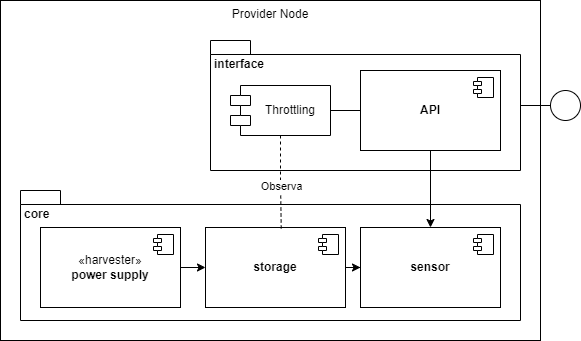
\includegraphics[width=0.75\linewidth]{Imagens/cap6/cap6providernode.png} 
	
	Fonte: elaborado pelo autor.
\end{figure}

Os elementos idealizados que constituem o dispositivo provedor são referentes aos seguintes componentes:
\begin{itemize}
	\item \textit{Power Supply}, representa a capacidade de coleta energética dos dispositivos, é caracterizado pela ação de fornecer os valores necessários para suas operações. No experimento, simula as características básicas de coleta de energia no decorrer de ciclos conforme descrito na Tabela \ref{table:cap6distribuicaonatal}. O componente atuará em paralelo a outras atividades realizadas pelo dispositivo. Caso o armazenamento do dispositivo esteja completamente cheio, ainda assim os valores de entrada serão entregues, caracterizando perdas. Por sua vez, o esgotamento energético do dispositivo não representa a incapacidade de receber novas entradas ofertadas e com isso, capacitar o dispositivo ao restabelecimento de suas funções.
	
	\item \textit{Storage} é responsável por receber os valores oferecidos pelo \textit{power supply} em função de suas características e capacidade de armazenamento, além disso, cabe a este componente oferecer reserva armazenada, com o objetivo de manter a disponibilidade energética do dispositivo sob certas circunstancias. A capacidade definida para o \textit{storage} do dispositivo deverá ser ajustada e deve representar a aderência da configuração proposta aos motivos que impõe a necessidade de um componente intermediário de armazenamento energético. Em função disso, os modos de operação podem ser estabelecidos pela distribuição proporcional à sua capacidade máxima.
	
	Para o experimento foi definido que os modos de operação utilizados deveriam incidir  apenas sobre o valor de recurso disponível no \textit{storage} do dispositivo, suficiente para expressão dos elementos taxonômicos. Foram obtidos pela proporcionalização da capacidade total de armazenamento presente no \textit{storage}. Sendo assim, a Tabela \ref{table:cap6:modos} apresenta os modos de operação para os dispositivos em relação a seu observável.
	
	
	\begingroup
	\begin{table}[htbp]
		
		\centering
		\caption{Modos de Operação dos Dispositivos.}
		\small
		%	\tabcolsep=0.05cm
		\begin{tabular}{ |c | c |}
			\hline
			Modo &Capacidade total do \textit{storage} $ (S) $\\
			\hline
			Abundante & $S \ge 70\% $\\\hline
			Atenção & $70\% > S \ge 50\% $\\\hline
			Alerta & $ 50\% > S \ge 10\%$ \\\hline
			Hibernando & $10\% > S \ge 0\%$  \\ \hline\addlinespace[1pt]
		\end{tabular}
		\label{table:cap6:modos}
		\\
		\footnotesize Fonte: elaborado pelo autor.
		
	\end{table}
	\endgroup
	
	
	 \item \textit{Sensor}, apesar de não estar presente diretamente na taxonomia, este componente é a representação das capacidades de atuação do dispositivo \acs{IoT}. Cabe a este componente realizar as operações necessárias conforme solicitado. Dentre as características presentes nos componentes em sensor esta a justificativa do gasto energético momentâneo mediante o estado que se encontra. Assim, é possível configurar um dispositivo com um ou mais sensores que proporcionem a representação de suas capacidades. Bastando para o experimento, a prévia implementação das especificações de custo operacional em cada estado possível dos sensores anexados. Assim, o dispositivo é capaz de simular a presença de um ou mais componentes e tem seu custo operacional em função da forma de uso de tais componentes.
	 
	 \item \textit{Interface} é o ponto de entrada para recebimento das solicitações, componente de interação com o dispositivo. O mecanismo de \textit{throttling} atuará acoplado a interface, controlando a vazão de atendimento a medida que permite ou bloqueia as solicitações recebidas em garantia de manter o modo de operação adequado em sincronismo ao estado das suas capacidades energéticas. Assim, uma vez atingido um limiar observado, instantaneamente o dispositivo poderá negar novas solicitações na interface, impedindo assim a propagação da mensagem que estimularia o seus demais componentes a atender uma demanda solicitada, através disso amortizando o gasto de recursos do dispositivo.
	 
\end{itemize}

\section{Instrumentalização}
\label{cap6:instrumentalizacao}
As ações executados para instrumentalização foram fundamentais para garantir a precisão e confiabilidade dos dados gerados durante a execução do experimento. O processo de decisão e escolha entre as ferramentas se deu com base na adequação à necessidade especifica do experimento realizado enquanto atende aos aspectos de coleta dos dados de forma objetiva sendo também essencial para as necessidades de visualização e análise dos resultados.

Para isso, o processo de coleta dos dados deve acontecer em intervalos regulares definidos previamente à execução do experimento, assim, todos os dados gerados são coletados simultaneamente em todos dispositivos dentro dos intervalos estipulados. Cabe também a necessidade de armazenamento desses dados capturados para análise posterior. Com essa demanda, justifica-se a opção de uso por uma ferramenta de uso livre, que fosse capaz de agregar em sua própria estrutura operacional aspectos para coleta de dados, armazenamento e consultas. A utilização da ferramenta Prometheus\footnote{Disponível em \url{https://prometheus.io/}.}, é fundamentada na sua reconhecida capacidade de atender especialmente os pontos elencados anteriormente, alem de ser aderente a estrutura criada para execução do experimento.

Portanto, de maneira transparente é embarcado ao dispositivo um cliente (\textit{Exporter}), este é responsável por expor os dados observáveis e de interesse para o experimento. Periodicamente, a cada 10 segundos, um agente externo chamado (\textit{Collector}) irá realizar chamadas com o objetivo de capturar os dados expostos pelo \textit{Exporter}. Assim, durante atividade de coleta, cabe ao agente coletor as ações de solicitar os dados providos no cliente para conversão e armazenamento destes na forma de séries temporal. 

Todos os dados recuperados pelo coletor são disponibilizados e mantidos em uma estrutura temporal para consultas no Prometheus. Graças a isso, qualquer visualizador capaz de realizar consultas em formato PromQL (\textit{Prometheus Query Language}) estará habilitado para visualizar execuções em andamento ou resgatar dados anteriores. A Figura \ref{fig:cap6instrumentalizacao} ilustra a dinâmica entre dispositivos e seus \textit{Exporters} embarcados e o agente externo coletor, e, por consequência, a disponibilidade dos dados para uma \textit{dashboard} de acompanhamento e posterior análise dos resultados. 

\begin{figure}[H]
	\centering
	
	\caption{Coleta e visualização da Execução do Experimento.}
	\label{fig:cap6instrumentalizacao}
	\noindent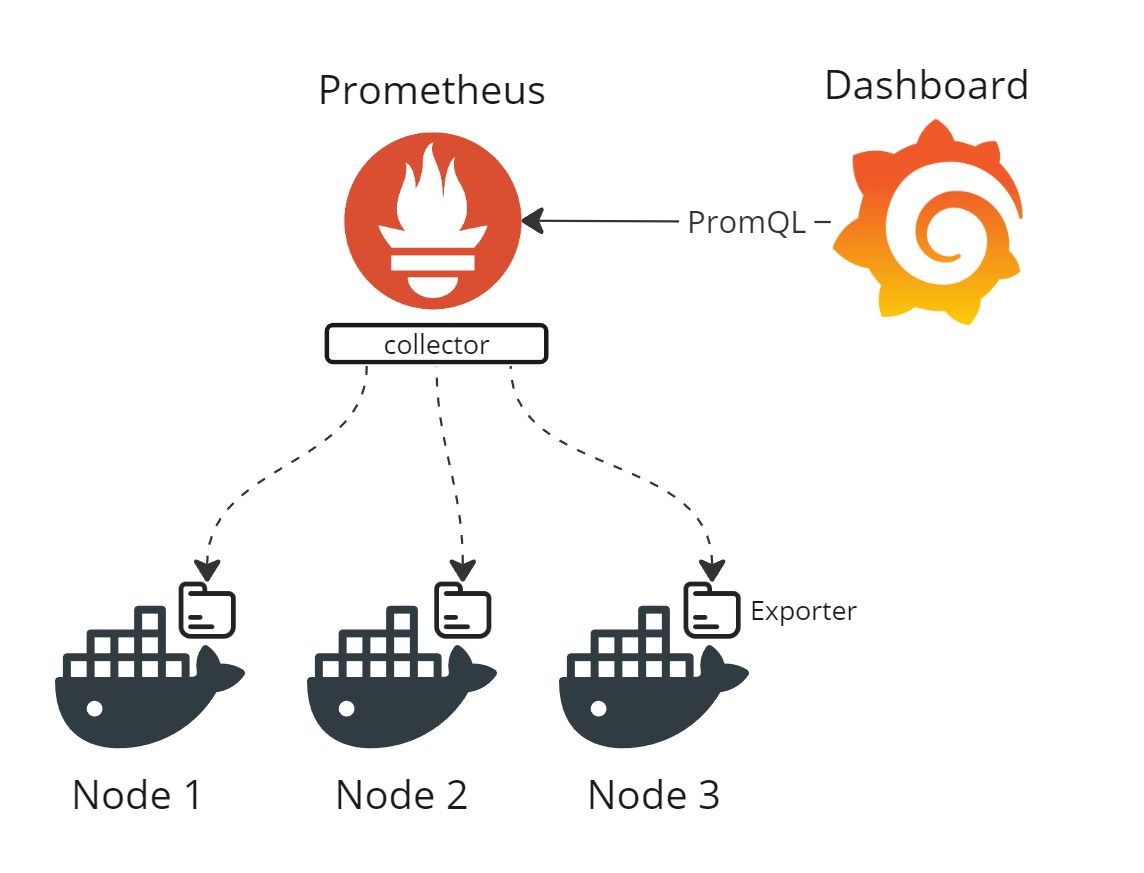
\includegraphics[width=0.75\linewidth]{Imagens/cap6/cap6instrumentalizacao.jpg} 
	
	Fonte: elaborado pelo autor.
\end{figure}


Com a necessidade de visualização dos dados durante execução, foi criado um quadro (\textit{dashboard}) para apresentar os resultados obtidos de forma gráfica. Logo, com o auxilio do Grafana\footnote{disponível em: \url{https://grafana.com/}}, uma plataforma aberta para análise e visualização de dados em quadros personalizáveis. Foi concebida essa interface de acompanhamento do experimento e a Figura \ref{fig:cap6bashboard} apresenta em aspecto a configuração dos quadros criados. Para avaliação posterior após a execução do experimento, os dados foram exportados, e dispostos em planilha eletrônica capaz de produzir os gráficos necessários para análise dos resultados. 

\begin{figure}[H]
	\centering
	
	\caption{Dashboard para visualização dos resultados.}
	\label{fig:cap6bashboard}
	\noindent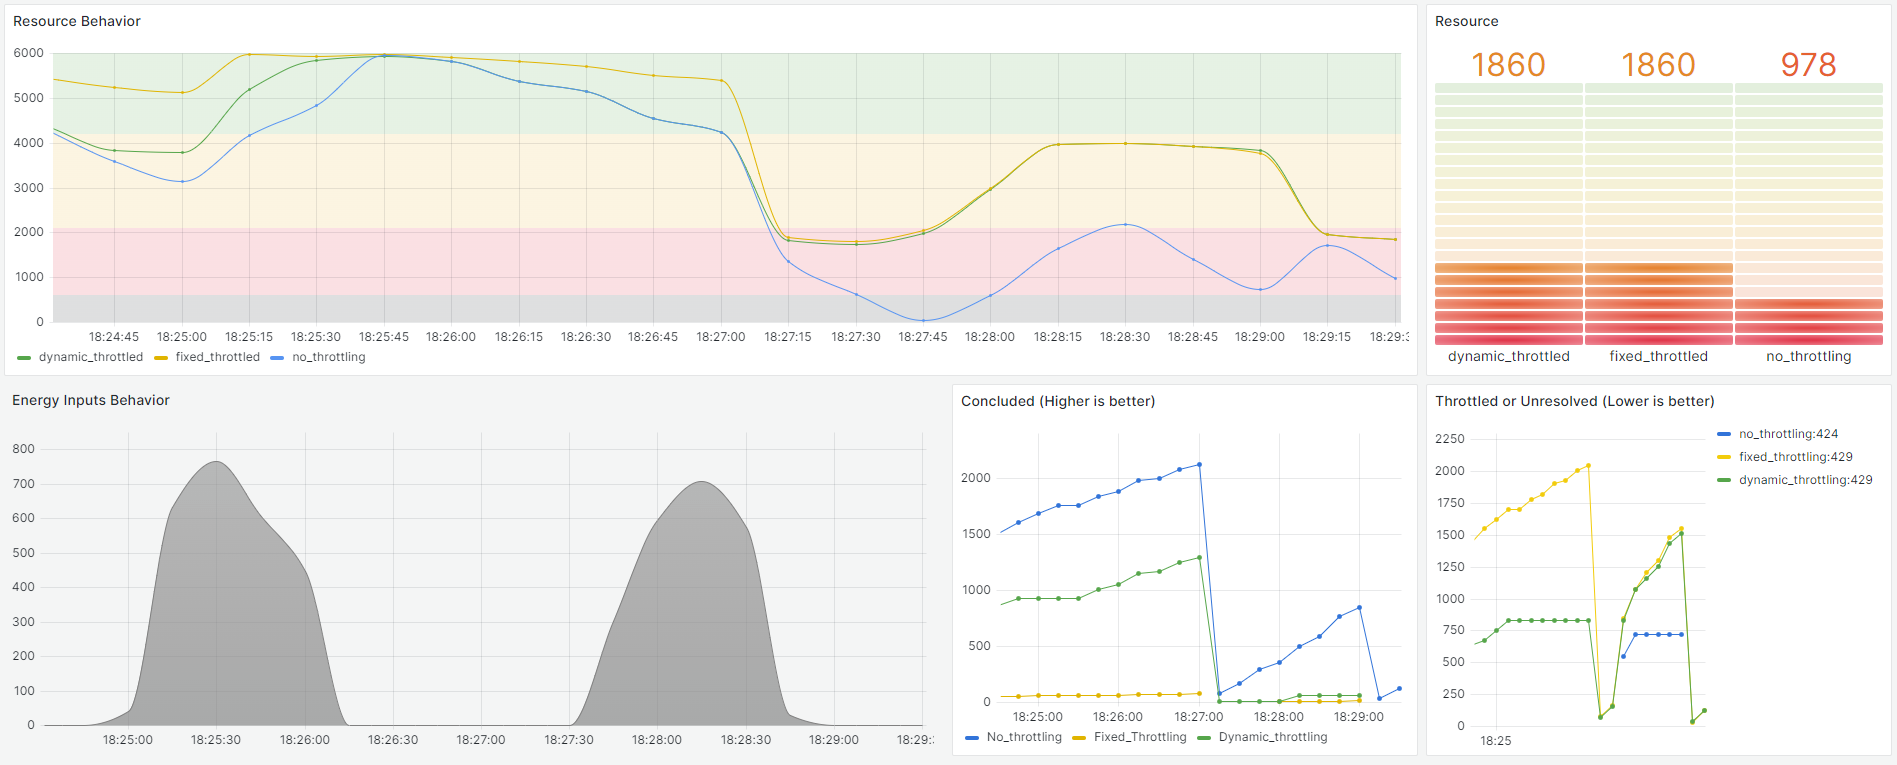
\includegraphics[width=1\linewidth]{Imagens/cap6/cap6dashboard.png} 
	
	Fonte: elaborado pelo autor.
\end{figure}

É pertinente ressaltar que os processos realizados para instrumentalização, em especial o \textit{exporter}, não exerce influência sobre a gasto energético simulado do dispositivo durante execução do experimento. Sua presença é transparente para a implementação, funcionando como um agente independente que não impacta nas dinâmicas energéticas colocadas em análise.

\section{Execução}
\label{cap6:execucao}

O estudo experimental foi realizado em etapas conforme descritos em referencia a Figura \ref{fig:cap6metodologia}, assim, as variáveis independentes descritas foram controladas para minimizar possível viés garantindo a consistência e replicabilidade do experimento. Durante a execução, os processos de instrumentalização atuaram em conformidade para que enquanto todos os dados necessários eram coletados, nenhuma variável externa pudesse influenciar nos resultados. Desta forma, as execuções contribuem para obtenção dos dados necessários para analisar e validar os resultados.

No inicio de uma execução, o \textit{storage} recebe o valor equivalente a sua capacidade máxima de armazenamento, a partir disso, os valores de oferta são disponibilizadas pelo \textit{power supply} e seguem a referencia apresentada na Tabela \ref{table:cap6distribuicaonatal}, assim, submetidos a medida que se inicia um novo ciclo $c_0, c_1,...,c_{23}$ relativos as jornada $J_1, J_2, ..., J_{12}$. Dado controle do experimento, a execução atende as características gerais de oferta de recursos com certa previsibilidade. Foram realizadas 3 execuções e seus resultados obtidos são em referencia dos mesmos valores fornecidos conforme descrito na Figura \ref{fig:cap6valoresofertados} na forma de variável independente.


Portanto, ao iniciar um ciclo $c$, o valor referente é entregue e, por sua vez, armazenado. Passados 6 segundos, um novo ciclo inicia-se encerrando o anterior em decorrência do novo valor ofertado. Este processo de iteração é referente aos ciclos de todas as jornadas e durará $\approx 1728 segundos$, tempo necessário para que o experimento apresente a atuação completa da dinâmica de estados e modos de operação possíveis.

\begingroup
\begin{table}[htbp]
	
	\centering
	\caption{Instanciação taxonômica para os dispositivos experimentados.}
	\small
	%	\tabcolsep=0.05cm
	\begin{tabular}{ c c c c c c c}
		\toprule
		Dispositivo & Operações & \textit{Throttling} & \multicolumn{4}{c}{Atuação}\\\cline{4-7}		
		& & & Limiar & Ciclos & Meios & Observáveis\\
		\midrule
		%		\hline
		 no-throttling  & $\approx 8640$ &Não & - & 288 & - & - \\
		fixed-throttling  & $\approx 8640$ &Sim & Fixo & 288 & Vazão & - \\
		 dynamic-throttling  & $\approx 8640$ &Sim & Adaptativo & 288 & Vazão & Reserva \\
		\bottomrule\addlinespace[2pt]
	\end{tabular}
	\label{table:cap6:dispositivosutilizados}
	\\
	\footnotesize Fonte: elaborado pelo autor.
	
\end{table}
\endgroup

O dispositivo 'no-throttling', representa o comportamento de dispositivos sem nenhum mecanismo de limitação das solicitações, seu objetivo principal é servir como base de comparação a medida que deverá atender todas as demandas solicitadas sem restrições previamente estabelecidas, com a observação de que caso seu valor armazenado em \textit{storage} seja completamente consumido, caracterizará esgotamento energético, incapacitando o dispositivo a atender qualquer tipo de solicitação.

Por sua vez, 'fixed-throttling'  e 'dynamic-throttling' foram implementados com a capacidade de limitar suas operações. Entretanto a atuação do mecanismo \textit{throttling} é distinta entre eles, para o 'fixed-throttling' é realizada restrição mediante limiar fixado apenas em razão da uma vazão de atendimento estipulada previamente sem observar adequação ao cenário energético ou privilégios do solicitante. Por sua vez, cabe a atuação do limitador presente em 'dynamic-throttling' atuar adaptativamente, assim como no anterior regulando a taxa de vazão de atendimento porém para este cabe observar as condições de sua reserva em \textit{storage}. Comportamento recorrente aos trabalhos relacionados ao contexto de atuação dos dispositivos. Sendo assim, a relação entre os modos de operação e como será o comportamento do limitador, quando presente, esta referenciado na Tabela \ref{table:cap6:expectativasolicitacoes}.

\begingroup
\begin{table}[h] \centering
	\caption{Expectativa de atendimento das solicitações ($sol$) por ciclo ($c$)}
	\small
%	\tabcolsep=0.05cm
	\begin{threeparttable}
	\begin{tabular}{ l c c c c c}
		\toprule
			Nome &
			\textit{Throttling   } & 
			\multicolumn{4}{c}{Modo de Operação}\\\cline{3-6}
			& &  \begin{tabular}{@{}c@{}} Abundante \\ {\tiny(\textit{S\tnote{*}} $\ge$ 70\% )} \end{tabular} &
			\begin{tabular}{@{}c@{}} Atenção \\ {\tiny(70\% > \textit{S} $\ge$ 50\%)} \end{tabular} &
			\begin{tabular}{@{}c@{}} Alerta \\ {\tiny(50\% > \textit{S} $\ge$ 10\%)} \end{tabular} &
			\begin{tabular}{@{}c@{}} Hibernando \\ {\tiny( 10\% > \textit{S} $\ge$ 0\%)} \end{tabular} \\
		\midrule
		 no-throttling &Não & 30 $sol/c$ & 30 $sol/c$ & 30 $sol/c$ & 30 $sol/c$ \tnote{**} \\
		 fixed-throttling & Sim & 15 $sol/c$ & 15 $sol/c$ & 15 $sol/c$ & 0 $sol/c$\\
		 dynamic-throttling & Sim & 30 $sol/c$ & 22 $sol/c$ & 15 $sol/c$ & 0 $sol/c$\\
		
		\bottomrule 
	\end{tabular}
	\begin{tablenotes}\footnotesize
		\item[*] \textit{S} representa o percentual do total energético armazenado em  \textit{storage} no momento observado.
		\item[**] Ao atingir 0\% o dispositivo estará esgotado e atenderá 0 $sol/c$.
	\end{tablenotes}
\end{threeparttable}
	\label{table:cap6:expectativasolicitacoes}
	\\
	\footnotesize Fonte: elaborado pelo autor.
\end{table}
\endgroup

Finalmente, o gasto dos recursos é obtido a partir da dinâmica de estados, ativo-inativo-hibernando e as condições para permanecer em um determinado estado conforme Figura \ref{fig:cap6maquinaestados}, sendo assim, dado um ciclo qualquer, o dispositivo que permanecer ativo durante todo tempo despenderá sua reserva de maneira  acentuada quando comparado a outro dispositivo que optou permanecer parcialmente inativo no contexto do ciclo em questão. Toda requisição realizada enquanto um dispositivo esteja em estado Hibernando, ou seja, sem reserva suficiente para manter-se operacional, será considerada não atendida em razão da indisponibilidade do dispositivo e quando sua reserva estiver completamente esgotada o dispositivo será considerado esgotado energeticamente.

\section{Avaliação dos Resultados}
\label{cap6:avaliacao}

Durante a avaliação dos resultados, examina-se em detalhes os valores obtidos a partir das execuções do experimento com o objetivo de validar o comportamento dos dispositivos a medida que refletem a completude dos elementos presentes na taxinomia enquanto demonstrama suficiência dos termos definidos nas classes para representar os dispositivos \acs{IoT} em computação dirigida à energia em função das ações do mecanismo de \textit{throttling}. Parte da avaliação se concentra também em apresentar descritivamente os dados coletados, a interpretação dos resultados e por fim, as limitações do estudo experimental.

\subsection{Descrição dos Dados Coletados}

A Figura \ref{fig:cap6valoresofertados}, apresenta o aspecto das características do ambiente onde o dispositivo esta inserido, do ponto de vista da distribuição dos valores ofertados. Estes, quantificaram a primeira variável independente e são utilizados para expressar as capacidades de coleta da abstração do sistema de coleta (\textit{power supply}) em um intervalo de tempo, sendo estes disponibilizados estritamente no inicio de cada ciclo. Sendo o primeiro valor no ciclo $c_{0}$ da jornada $J_1$ e, por sua vez, o ultimo transmitido no inicio do ciclo $c_{23}$ da jornada $J_{12}$. Decorrido o tempo disposto para o ultimo ciclo da jornada $J_{12}$, finda-se a execução do experimento.

\begin{figure}[H]
	\centering
	
	\caption{Característica do ambiente de simulação e valores coletados.} 
	\label{fig:cap6valoresofertados}
	\noindent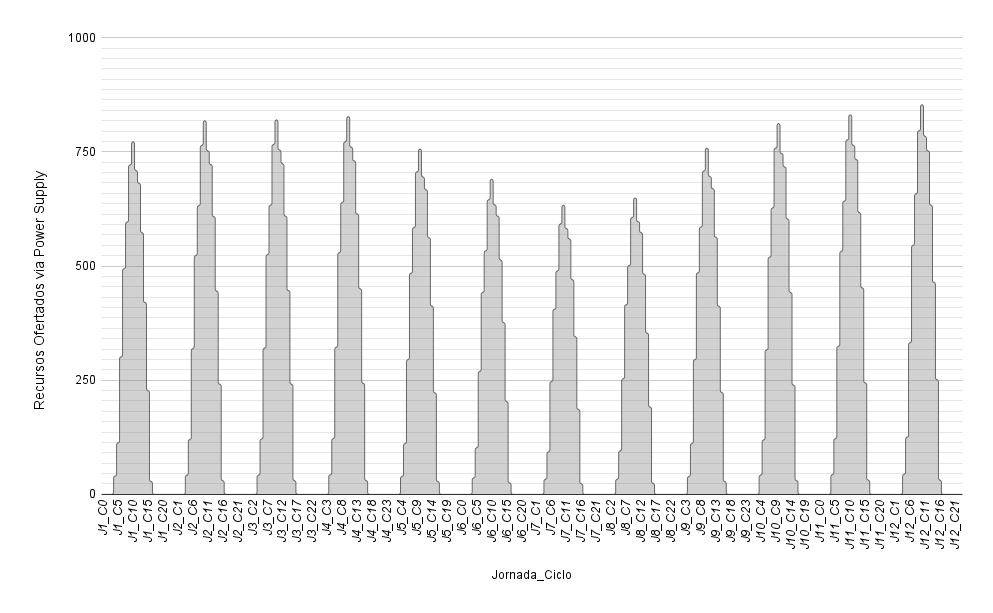
\includegraphics[width=1\linewidth]{Imagens/cap6/cap6valoresofertados.png} 
	
	Fonte: elaborado pelo autor.
\end{figure}

Diante da natureza do experimento, toda execução obtêm o mesmo comportamento da oferta energética conforme distribuição definida. Assim os valores já seguem definidos antes da execução e não sofrem impacto diante das eventos externos no contexto de uma ou outra execução. Representa um ambiente e suas características em termos de previsibilidade energética e capacidade de controle \cite{sudevalayam_energy_2011}, além disso, é garantido ao dispositivo receber este valor mesmo que esteja momentaneamente esgotado, pois não foram encontrados indícios suficientes à restrições do evento de oferta energética no contexto de computação dirigida à energia.

A segunda variável independente utilizada, representa as solicitações disparadas contra a interface do dispositivo provedor. Este estimulo caracteriza-se pela classe Operações e representam os movimentos de mensagens para consumo e demanda submetida ao dispositivo. Portanto, ao atender-las, o provedor deverá intensificar seu consumo energético, pois encontra-se em estado ativo, demandando mais recursos. Isso implica que, à medida que a quantidade das solicitações atendidas aumenta, o consumo de energia do provedor também aumentará proporcionalmente, podendo resultar em impacto significativo na disponibilidade do dispositivo em relação com seu desempenho energético. A Tabela \ref{table:cap6:execucaocaracteristicas}, apresenta os valores utilizados para as requisições em cada execução do experimento. A precisão indica a distribuição da relação entre total de solicitações em cada execução em referencia para 12 jornadas descrito na Seção \ref{cap6:execucao}.

\begingroup

\begin{table}[h]
	
	\centering
	\caption{Solicitações realizadas}
	\begin{threeparttable}
	\begin{tabular}{ l c c c c }
		\toprule
		&   & \multicolumn{3}{c}{Solicitações ($sol$)}\\\cline{3-5} & Duração&
		\begin{tabular}{@{}c@{}} Execução 1\end{tabular} & \begin{tabular}{@{}c@{}} Execução 2\end{tabular} & \begin{tabular}{@{}c@{}} Execução 3\end{tabular}\\
		\bottomrule
		1 ciclo  				& 6 $seg$ 	& 29,875 	& 29,86 & 29,88 \\
		1 Jornada (24 ciclos)  	& 144 $seg$	& 717 & 716,75 &  717,16\\
		12 Jornadas  			& 1728 $seg$& 8604  & 8601 & 8606 \\
		\bottomrule
	\end{tabular}

	\end{threeparttable}
	\label{table:cap6:execucaocaracteristicas}
	\\
	\footnotesize Fonte: elaborado pelo autor.
	
\end{table}
\endgroup


Ao finalizar uma execução, as variáveis dependentes obtidas são colhidas para avaliação: a quantidade total de solicitações atendidas, que expressam a atuação do mecanismo de \textit{throttling}; a quantidade de solicitações impedidas mediante indisponibilidade do dispositivo por esgotamento energético, que motivam ao pensamento crítico de como o agente limitante poderia ter se atuado ou não. Para analisar a diferença na quantidade de solicitações atendidas, é necessário contrapor dados de reserva em \textit{storage} com os valores ofertados pelo \textit{power supply}, assim obtendo visão completa do comportamento do dispositivo \acs{IoT} enquanto atuação de limitadores.	

Ainda sobre os dados coletados, ao final de cada execução é obtido o total de requisições atendidas evidenciando como as características da ação dos agentes limitantes apenas sobre a performance dos dispositivos. Na Figura \ref{fig:cap6solicitacoesatendidas}, é possível comparar o desempenho de dispositivos sob a ponto de vista das solicitações atendidas. Toda via, é preciso análise cuidadosa sob o ponto de vista da performance, seu objetivo não é apresentar qual comportamento foi mais eficiente mas trazer a superfície o impacto das características delegadas a cada dispositivo enquanto instancias da taxonomia proposta.

\begin{figure}[H]
	\centering	
	\caption{Quantidade de solicitações atendidas por dispositivo.} 
	\label{fig:cap6solicitacoesatendidas}
	\noindent\includegraphics[width=0.8\linewidth]{Imagens/cap6/cap6solicitaçoesatendidas_execs.png} 
	
	Fonte: elaborado pelo autor.
\end{figure}


Apenas o dispositivo "no-throttling" apresentou em seu resultado um valor de indisponibilidade em função de esgotamento energético, de modo geral a Tabela \ref{table:cap6:quadrogeralobtido} apresenta os valores obtidos em um quadro geral, mais uma vez, seus resultados evidenciam as características do agente limitante, reduzindo a capacidade de atendimento em função da proteção contra o esgotamento energético, representado na tabela pelo valor de indisponibilidade.

\begingroup
\begin{table}[H]
	\centering
	\caption{Quadro das solicitações realizadas aos dispositivos}
	\begin{tabular}{|c|c|c|c|c|c|}
		\hline
		\multirow{2}{*}{Execução} & 
		\multirow{2}{*}{Dispositivo} &
		\multicolumn{4}{c|}{Solicitações}  \\\cline{3-6}\addlinespace[1pt]
		& & realizadas&  atendidas & indisponíveis  & \% indisponíveis \\
		\hline\addlinespace[1pt]
		\multirow{3}{*}{1} 	& no-throttling 	& 8604 &  7043	& 1561 	 	& 0.1814\\
							& fixed-throttling 	& 8604 &  3414	& 0 		& -\\
							& dynamic-throttling & 8604 & 5098 & 0 		&-\\
		\hdashline\addlinespace[1pt]
		\multirow{3}{*}{2}	& no-throttling 	& 8601 & 7105	& 1496  & 0.1739\\
							& fixed-throttling 	& 8601& 3436	& 0  & -\\
							& dynamic-throttling & 8601 & 5118	& 0  &-\\
		\hdashline\addlinespace[1pt]
	   \multirow{3}{*}{3}  & no-throttling & 8606 & 7105& 1504 &0.1747\\
	   	& fixed-throttling & 8606 &3441 & 0& -\\
	   	& dynamic-throttling & 8606 & 5123& 0&-\\
		\hline

	\end{tabular}
		\label{table:cap6:quadrogeralobtido}
		\\
		\footnotesize Fonte: elaborado pelo autor.
\end{table}
\endgroup

Parte da análise é obtida ao observar o gráfico de comportamento referente às capacidades energéticas  observadas no \textit{storage} do dispositivo. A Figura \ref{fig:cap6recortecomportamentostorage} apresenta um recorte dos dados, oferecendo informações suficientes para inferências sobre a dinâmica entre a coleta e a forma de consumo de recursos por todos os dispositivos envolvidos. Essa visualização permite identificar alguns padrões de consumo e tendências de comportamento do dispositivo especialmente nas áreas em destaques que apresentaram oferta minima ou inexistente de recurso disponibilizado.

\begin{figure}[H]
	\centering	
	\caption{Recorte do comportamento da oferta e uso dos recursos durante execução.} 
	\label{fig:cap6recortecomportamentostorage}
	\noindent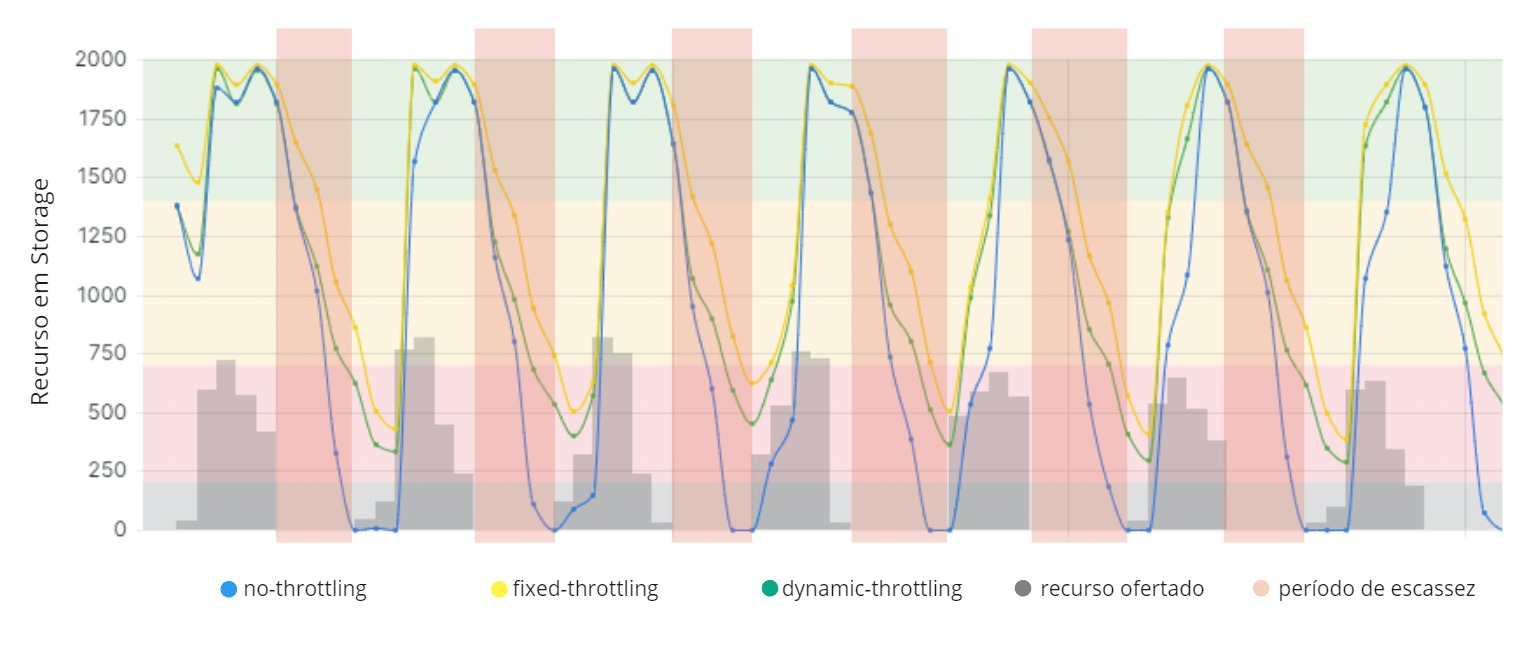
\includegraphics[width=1\linewidth]{Imagens/cap6/cap6recortecomportamentostorage.jpg} 
	
	Fonte: elaborado pelo autor.
\end{figure}

Finalmente, a análise realizada sobre a Figura \ref{fig:cap6recortecomportamentostorage} permite a visualização do recorte ampliado de sete jornadas, representa o claro comportamento dos dispositivos enquanto a atuação é restrita ou não em cada modo de operação referente a sua condição apresentada em \textit{storage} e os limiares definidos na Tabela \ref{table:cap6:modos}, este processo é notável através da clara amortização intensificada na tendencia das linhas de consumo enquanto o valor de recurso encontra-se dentro de cada modo, representado nas faixas horizontais destacadas na relação de cores.


\subsection{Interpretação dos Resultados}
\begin{comment}
	Descreva os resultados dos testes de uma maneira que seja compreensível para o leitor. Discuta se os resultados foram estatisticamente significativos e o que isso significa em termos do seu experimento.
\end{comment}

Com as execuções realizadas, é possível conceber a completude da categorização taxonômica e sua organização. Ao instanciar os dispositivos do ponto de vista de suas classes,  é possível observar como se comportam em virtude das características dos fatores energéticos aos quais estão expostos, conforme categorização observada na revisão apresentada no Capítulo \ref{cap:cap3}. Através dessas execuções, podemos analisar de que forma a energia ofertada durante o experimento impactou no desempenho dos dispositivos permitindo uma compreensão profunda dos seus comportamentos e limitações em ambientes, em especial com características preditivas e pouco controladas.

Ao categorizar um dispositivo \acs{IoT} em computação dirigida à energia, é preciso fazer menção sobre o papel que este irá desempenhar. Para isso, o experimento atuou gerando um mesmo cenário para que os diferentes agentes examinados pudessem cumprir o papel de provedor de informações de sensores. Assim, os resultados obtidos, descrevem a importância dos elementos categorizados em função das características encontradas nos trabalhos relacionados à dispositivos para computação dirigida à energia. Na medida que observam-se o comportamento simulado dos fatores energéticos e os impactos observados a busca por evitar um esgotamento energético.

Sobre a capacidade de atender solicitações, a análise do uso de recursos utilizados pelo dispositivo 'no-throttling' na Figura \ref{fig:cap6nothrottling} destaca que a continuidade no seu desempenho para atender solicitações é fortemente impactada pelos valores energéticos coletados. Por não possuir nenhum agente limitador experimentado, o dispositivo tem a capacidade de utilizar seus recursos de forma irrestrita, mesmo em cenários de escassez. No entanto, isso pode conduzi-lo à estado de esgotamento, onde ele perde a capacidade de realizar qualquer ação, mesmo um eventual contingenciamento dos efeitos da indisponibilidade, o que pode ter consequências graves. Portanto, mesmo em cenário de dispositivos com capacidade de armazenamento energético, se faz necessária a aplicação de politicas de limitação de uso em ciclos, em acordo com \acs{SLA} estabelecido indicando os termos de atuação para os quais os dispositivos \acs{IoT} deveram atender.

\begingroup
\begin{figure}[htb]
	
	\centering
	\caption{Aqui vou colocar uma figura para isolar o comportamento do no-throttling.}
	\label{fig:cap6nothrottling}
	\noindent\includegraphics[width=0.3\linewidth]{example-image} 
	
	Fonte: elaborado pelo autor.
\end{figure}
\endgroup


Posteriormente, ao instanciar os dois dispositivos com diferentes limitadores, com o pretexto de validar a aderência dos conceitos classificados na taxonomia proposta. Os dados obtidos oriundos da experimentação colaboram com o entendimento dos elementos envolvidos no processo de concepção do que compreende minimamente um dispositivo \acs{IoT} encontrado em computação dirigida à energia. Sobretudo é percebido também necessidade de implementar os mecanismos de limitação para lidar com os aspectos de disponibilidade.

Em relação ao comportamento esperado dos agentes, nota-se que o mecanismo \textit{throttling} exerceu influência ativa contribuindo para adequação de comportamento do dispositivo provedor, sobretudo quando considera a observação dos aspectos dos recursos energéticos envolvidos, necessários para alcançar um grau de disponibilidade estimada presente em um acordo de nível de serviço. Ainda sobre estes termos, confrontam-se o desempenho obtido pelos dispositivos 'fixed-throttling' e 'dynamic-throttling', na Figura \ref{fig:cap6fixedxdynamic}, correspondendo a necessidade da atuação do mecanismo limitador em função da observação dos termos classificados como Observáveis na taxonomia.

Graças a isso, é possível perceber que o dispositivo 'fixed-throttling' obteve menor variação de sua reserva energética, se valendo da periodicidade da condição de oferta, teve o \textit{throttling} atuando fixamente durante os ciclos, e assim, de maneira constante consumiu seus recursos ao passo que também atendia as solicitações em termos dos limites da taxa de vazão sobre os meios desse dispositivo provedor sem observar necessariamente nenhum critério observável categorizado.

Esta abordagem foi especialmente útil a medida que geram indicios para caráter opcional sobre um termo especifico, dado que o dispositivo experimentado com limiar de atuação fixo manteve-se operacional. Todavia, é preciso atenção sobre essa afirmação, pois dada o universo de atuaçao \acs{IoT} os mecanismos de limitação de operações frequentemente precisam considerar características específicas dos dispositivos na forma de observáveis e do ambiente, sendo em muitos casos, considerado precipitado apenas limitar sua taxa de vazão (\textit{Throughput}) quaisquer que sejam os valores. Para conhecimento, nenhum trabalho citado apresentou solução puramente baseada nos meios de atuação do mecanismo \textit{throttling} pois mesmos os que buscaram previsibilidade de demanda, se utilizam de outros fatores, os observáveis, para justificar seu comportamento.
 
\begingroup
\begin{figure}[htb]
	
	\centering
	\caption{Comparação comportamento das estratégias de throttling aplicadas.}
	\label{fig:cap6fixedxdynamic}
	\noindent\includegraphics[width=0.3\linewidth]{example-image} 
	
	Fonte: elaborado pelo autor.
\end{figure}
\endgroup

Ainda sobre a discussão a respeito da análise de observáveis, a Figura \ref{fig:cap6fixedxdynamic} apresenta, mediante execução dos agentes instanciados, a diferença de comportamento do dispositivo 'dynamic-throttling' em relação à outra implementação com limites fixos, que foi proporcionado pela capacidade incrementada ao \textit{throttling} em observar os fatores de sua reserva energética. Com isso apoiou o dispositivo em função da capacidade de gerenciamento sobre seu comportamento, fundamental para gerar capacidade adaptativa para os ciclos. Assim, apesar dos momentos de escassez, o dispositivo foi capaz de manter-se disponível energeticamente e ainda obter o total de solicitações atendidas superiores aos obtidos pela abordagem do dispositivo que utiliza limitador fixo em função unicamente da vazão de atendimento. Colaborando com o entendimento sobre a necessidade de categorizar os observáveis quando na atuação do mecanismo limitador.
 
Finalmente, as instancias experimentadas apresentam, evidenciados pelo comportamento nos resultados obtidos, as referências aos atributos listados para o uso de throttling como atuador em busca de atender critérios de disponibilidade, especialmente para os dispositivos \acs{IoT} presentes em computação dirigida à energia. Com isso, gerando indícios da completude sobre os elementos ligados taxonomicamente aos fundamentos de atuação do \textit{throttling}, mediante analise cuidadosa dos termos de serviço necessários para definir uma configuração de atuação colaborando para o objetivo de manter os dispositivos disponíveis.



\subsection{Limitações do Estudo}
\begin{comment}
	Reconheça quaisquer limitações do seu estudo que possam ter afetado os resultados. Isso pode incluir limitações metodológicas, questões de amostragem, viéses potenciais ou qualquer outra consideração importante.
\end{comment}


As limitações do experimento preliminar, passa especialmente pela não examinação de alguns cenários. Apesar de considerados na taxonomia, o experimento não explorou as características de transmissão inerentes à dispositivos \acs{IoT}, presentes em alguns trabalhos visitados \cite{gong_sleep_2022}. Outro fator não examinado foi diretamente ligado à capacidade de depreciação prevista por \citeonline{shen_energy-efficient_2019} uma vez que os dispositivos instanciados apresentam apenas um componente do tipo sensor. Alternativamente o comportamento dos estados (Ativo-Inativo-Hibernando) podem ser descritos em função de outros componentes presentes, essenciais como previstos pelo autor. Em todo caso, na análise experimental não foram realizadas menções diretas a capacidade de ajustar o consumo energético dos sensores.

Algumas características da taxonomia não foram cobertas em sua totalidade no experimento, não é possível examinar o ponto de vista do consumo energético dos agentes enquanto clientes por exemplo. Em todo caso, foi garantido que os elementos presentes fossem minimamente utilizados, mesmos que não possuam observações relevantes em virtude dos termos experimentados.





 